\documentclass[11pt,a4paper]{article}

\usepackage[T1]{fontenc}
\usepackage[utf8]{inputenc}
\usepackage{lmodern}
\usepackage{amssymb}
\usepackage[margin=22mm]{geometry}
\usepackage{xcolor}
\usepackage{microtype}
\DisableLigatures{encoding=T1,family=tt*}
\usepackage{enumitem}
\usepackage{booktabs}
\usepackage{tabularx}
\usepackage{listings}
\usepackage{tikz}
\usetikzlibrary{arrows.meta,positioning}
\usepackage{fancyhdr}
\usepackage{hyperref}

\definecolor{ZipperInk}{HTML}{17212B}
\definecolor{ZipperBlue}{HTML}{176B87}
\definecolor{ZipperLight}{HTML}{EEF6F8}
\definecolor{CodeBackground}{HTML}{F5F7F8}
\definecolor{AgentBackground}{HTML}{F2F0F7}
\definecolor{CodeComment}{HTML}{58715D}
\definecolor{CodeKeyword}{HTML}{7A3E9D}
\definecolor{WarningBorder}{HTML}{B7791F}
\definecolor{ZipperGreen}{HTML}{2F855A}

\hypersetup{
  colorlinks=true,
  linkcolor=ZipperBlue,
  urlcolor=ZipperBlue,
  citecolor=ZipperBlue,
  pdftitle={Your First ZipperGen Workflow},
  pdfauthor={The ZipperGen Authors}
}

\pagestyle{fancy}
\fancyhf{}
\lhead{Your first ZipperGen workflow}
\rhead{Draft, approve, send}
\cfoot{\thepage}
\setlength{\headheight}{14pt}

\setlist[itemize]{topsep=4pt,itemsep=2pt}
\setlist[enumerate]{topsep=4pt,itemsep=3pt}
\setlength{\parindent}{0pt}
\setlength{\parskip}{6pt}

\lstset{
  basicstyle=\ttfamily\small,
  backgroundcolor=\color{CodeBackground},
  frame=single,
  rulecolor=\color{black!18},
  breaklines=true,
  breakatwhitespace=false,
  columns=fullflexible,
  keepspaces=true,
  showstringspaces=false,
  upquote=true,
  keywordstyle=\color{CodeKeyword}\bfseries,
  commentstyle=\color{CodeComment},
  stringstyle=\color{ZipperBlue},
  numbers=none
}

\lstdefinestyle{shell}{
  language=bash,
  numbers=none
}

% What the coding agent says, visually distinct from what you type.
\lstdefinestyle{agent}{
  language={},
  backgroundcolor=\color{AgentBackground},
  basicstyle=\ttfamily\footnotesize,
  numbers=none
}

\lstdefinestyle{pane}{
  basicstyle=\ttfamily\scriptsize,
  numbers=none,
  aboveskip=2pt,
  belowskip=2pt
}

% Two terminals side by side, used only where the handoff is the point. At
% this width each pane is narrow, so long output belongs in a full-width
% listing instead.
\tikzset{
  zgstage/.style={
    draw=ZipperBlue,
    fill=ZipperLight,
    very thick,
    rounded corners=2.5pt,
    align=center,
    minimum height=11mm,
    inner sep=4pt,
    font=\small
  },
  zgflow/.style={-{Latex[length=2.2mm,width=1.5mm]}, thick, draw=ZipperBlue}
}

\newenvironment{notebox}[1]
{\begin{center}\begin{minipage}{0.94\linewidth}
 \color{ZipperInk}\hrule\vspace{5pt}\textbf{#1}\par\smallskip}
{\vspace{5pt}\hrule\end{minipage}\end{center}}

\newenvironment{warningbox}[1]
{\begin{center}\begin{minipage}{0.94\linewidth}
 \color{WarningBorder}\hrule\vspace{5pt}
 \color{ZipperInk}\textbf{#1}\par\smallskip}
{\vspace{5pt}\color{WarningBorder}\hrule\end{minipage}\end{center}}

\title{\color{ZipperInk}\Huge\textbf{Your First ZipperGen Workflow}\\[5pt]
\Large Draft a reply, ask a person, then send}
\author{The ZipperGen Authors}
\date{Tutorial edition: 8 August 2026}

\begin{document}

\maketitle

\begin{abstract}
You will build a small application that watches a mailbox, asks a language
model to draft a reply to each message, and asks \emph{you} to approve it
before anything is sent. It does not stop on its own. It is a service, and the
last section leaves it running on a server. It is short enough to read in
one sitting, and it already contains everything that makes ZipperGen worth
using: two participants, a model call, an explicit human decision, a branch
that only the decider takes, and a loop that keeps the whole thing alive.

There is no separate ZipperGen development environment to learn. You work in an
ordinary directory with an ordinary command line, and, if you like, a coding
agent such as Claude Code or Codex. This tutorial shows both, and is honest about which parts
need a person.
\end{abstract}

\section{What you are building}

\begin{center}
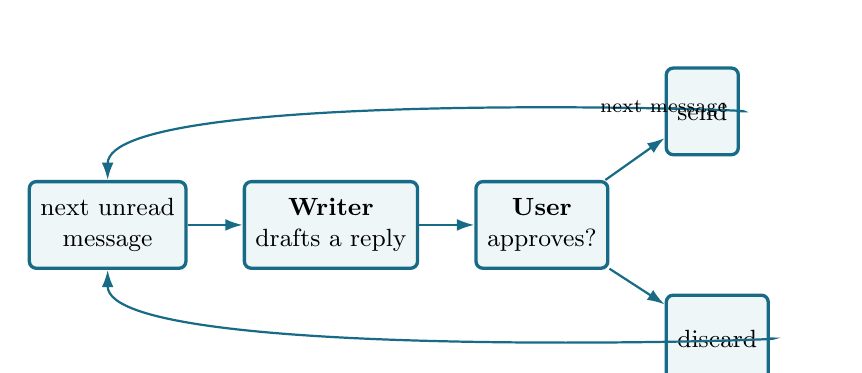
\begin{tikzpicture}[node distance=7mm]
  \node[zgstage] (msg)   {next unread\\message};
  \node[zgstage, right=of msg] (draft) {\textbf{Writer}\\drafts a reply};
  \node[zgstage, right=of draft] (ask) {\textbf{User}\\approves?};
  \node[zgstage, above right=3mm and 7mm of ask] (send) {send};
  \node[zgstage, below right=3mm and 7mm of ask] (drop) {discard};
  \draw[zgflow] (msg) -- (draft);
  \draw[zgflow] (draft) -- (ask);
  \draw[zgflow] (ask) -- (send);
  \draw[zgflow] (ask) -- (drop);
  \draw[zgflow] (send.east) .. controls +(right:8mm) and +(up:12mm) ..
    node[right,font=\scriptsize,pos=0.35]{next message} (msg.north);
  \draw[zgflow] (drop.east) .. controls +(right:8mm) and +(down:12mm) .. (msg.south);
\end{tikzpicture}
\end{center}

It then waits for the next message, and does it again. Nothing ends the loop,
which is what makes this a service rather than a script.

Concretely, you want this to happen:

\begin{notebox}{Incoming message}
Could we move our meeting to Thursday afternoon?

\smallskip
\textbf{Proposed reply}\\
Thursday afternoon works for me. How about 3pm?

\smallskip
\texttt{[ Send ] [ Reject ]}
\end{notebox}

Two participants exchange messages, one of them is a person, and what happens
next depends on what that person says. That is a coordination problem, and it
is the kind of thing ZipperGen exists to make readable.

\begin{notebox}{What you need}
\begin{itemize}
  \item Python 3.11 or newer and ZipperGen installed.
  \item Nothing else for the first two thirds. The model is mocked and the
        approval happens in your terminal.
  \item For the last section, a Telegram bot token, if you want the approval to
        arrive on your phone.
\end{itemize}
\end{notebox}

\section{Create the project}

\begin{lstlisting}[style=shell]
mkdir email-approval && cd email-approval
zippergen init
\end{lstlisting}

\begin{lstlisting}
ZipperGen project: email-approval
  zippergen.toml     created
  specification.md   created
  AGENTS.md          created
  CLAUDE.md           created
\end{lstlisting}

\begin{notebox}{\texttt{zg} is short for \texttt{zippergen}}
Both commands are installed and do the same thing. The rest of this tutorial
uses \texttt{zg}, because the commands you type often are the ones worth
shortening.
\end{notebox}

That is the whole of project creation. It writes four files and stops: it asks
you nothing, and it configures nothing.

\begin{itemize}
  \item \texttt{zippergen.toml} is the project's visible configuration. It is
        committed, and it never contains a credential.
  \item \texttt{specification.md} says what the workflow is meant to do, in prose.
  \item \texttt{AGENTS.md} tells a coding agent to run
        \texttt{zippergen skill} before touching workflow code.
  \item \texttt{CLAUDE.md} points Claude Code at the same shared instructions.
\end{itemize}

\section{Describe what you want}

You can write the workflow yourself, and the next section shows the code. But the
intended path is to say what you want in ordinary language. Open a coding agent
in this directory:

\begin{lstlisting}[style=shell]
claude
\end{lstlisting}

and ask for it:

\begin{lstlisting}[style=agent]
> Build a ZipperGen workflow that watches a mailbox directory, asks an LLM
  to draft a short reply to each new message, and asks me to approve it
  before it is sent. It should keep running and wait for the next message.
\end{lstlisting}

The agent reads \texttt{AGENTS.md}, which points it at \texttt{zg skill}.
Those are ZipperGen's own instructions for how to write a workflow, what to check, and
what never to touch. It writes the files, then checks its work with the same
commands you would use:

\begin{lstlisting}[style=agent]
I created specification.md and workflow.py.

  $ zg validate
  Workflow email_approval: valid

Two participants, User and Writer, and one decision that the User owns:
whether to send the draft. Ask me to change anything.
\end{lstlisting}

That is the shape of the whole thing. You describe what you want. The agent
edits ordinary files and uses ZipperGen's actions to check them. Nothing
happened that you could not have done by hand, and everything it did is visible
in the directory.

\begin{notebox}{Where the skill comes from}
\texttt{zg skill} prints instructions that ship inside the package, so they
match the version you have installed. They are ordinary prose in the
repository, not generated text. You can read them, and you can disagree with
them.
\end{notebox}

\section{What comes out}

Visible, readable Python. This is the whole coordination:

\begin{lstlisting}[language=Python]
@workflow
def email_approval() -> int:
    User: message = next_unread_message()
    while message @ User:
        User(message) >> Writer(message)
        Writer: draft = draft_reply(message)
        Writer(draft) >> User(draft)
        User: approved = approve_reply(draft)
        if approved @ User:
            User: handled = send_reply(draft, handled)
        else:
            User: handled = discard(handled)
        User: message = next_unread_message()
    return handled @ User
\end{lstlisting}

Read it top to bottom and you have the entire message order. Five things are
worth noticing.

\texttt{User(message) >> Writer(message)} is a message. The left side sends,
the right side receives, and the names in brackets say which variables carry
the value.

\texttt{Writer: draft = draft\_reply(message)} is an action performed by one
participant. \texttt{draft\_reply} is an \texttt{@llm} action, which is a model
call with a prompt and a declared output.

\texttt{User: approved = approve\_reply(draft)} is a \texttt{@human} action. It
stops and waits for a person.

\texttt{if approved @ User} is a decision, and the \texttt{@ User} says who
makes it. That annotation is the important one, and the next section shows why.

\texttt{while message @ User} is a loop, owned the same way. The
\texttt{User} decides each round whether there is another message to handle.
\texttt{next\_unread\_message} waits until there is one, so in practice that
decision is always yes and the workflow never finishes. That is the point.

\begin{notebox}{One action hides the awkward part}
Mailboxes are fiddly: what to do when nothing is unread, how to avoid handling
the same message twice, whether to poll or block. All of it sits behind
\texttt{next\_unread\_message}, whose contract is one sentence: \emph{return the
next message, waiting if there is none}. Here it takes the oldest
\texttt{.txt} file from \texttt{mailbox/} and renames it \texttt{.done}, so no
message is handled twice even after a crash. The coordination above does not
change when you point it at a real inbox.
\end{notebox}

\section{Check it yourself}

Everything the agent ran, you can run:

\begin{lstlisting}[style=shell]
zg validate
\end{lstlisting}

\begin{lstlisting}
Workflow email_approval: valid
OK   lifelines: 2 unique lifeline(s): Writer, User
OK   projection Writer: SeqStmt
OK   projection User: SeqStmt
OK   deployment declaration: 0 field(s), 0 package(s), 0 setup step(s)
OK   canonical rendering: global and local code views rendered successfully
\end{lstlisting}

\texttt{validate} loads the module, projects the protocol for every
participant, and renders it back. If it passes, the workflow is well formed and
the deadlock-freedom guarantee applies to it.

There is no privileged mode here. The agent and you have the same commands.
Credentials are the exception, and you supply those yourself. The rest of
this tutorial mixes both: asking the agent when a question is easier to say
than to type, and running commands directly when they are short.

\section{The moment that matters}

The workflow has one decision and the \texttt{User} makes it. Rather than
reading the code again, ask:

\begin{lstlisting}[style=agent]
> What does the Writer actually run?
\end{lstlisting}

\begin{lstlisting}[style=agent]
  $ zg show --agent Writer

  @role('Writer')
  def email_approval__Writer() -> None:
      while recv_decision('User'):
          message = recv('User')
          draft = draft_reply(message)
          send('User', draft)

The Writer is told each round whether to keep going, then drafts one
reply. It is never told whether the reply was sent: the User owns the
approval decision, and the Writer takes no part in it.
\end{lstlisting}

Run it yourself and you get the same four lines. Now compare the
\texttt{User}, who owns both the loop and the decision:

\begin{lstlisting}[style=shell]
zg show --agent User
\end{lstlisting}

\begin{lstlisting}[language=Python]
@role('User')
def email_approval__User() -> int:
    message = next_unread_message()
    while message:
        send_decision('Writer', True)
        send('Writer', message)
        draft = recv('Writer')
        approved = approve_reply(draft)
        if approved:
            handled = send_reply(draft, handled)
        else:
            handled = discard(handled)
        message = next_unread_message()
    else:
        send_decision('Writer', False)
    return handled
\end{lstlisting}

\begin{notebox}{The Writer has no approval branch}
Nobody wrote either of those lines. Put the two programs side by side and the
\texttt{User} does something for each of its two control structures, while the
\texttt{Writer} does something for only one of them.

The loop, the \texttt{Writer} must know about: it has work inside it, so the
\texttt{User} tells it every round whether to continue, and tells it once more,
at the end, not to. That is the \texttt{send\_decision} in the
\texttt{else}.

The approval, the \texttt{Writer} must \emph{not} know about: it does nothing
in either branch, so the decision is erased from its program entirely. It
cannot wait on it, disagree with it, or deadlock against it.

In a hand-written multi-agent system this is exactly where the bugs live: one
agent waits for a message the other decided not to send. Here the question does
not arise, because the projection worked out who needed telling and who did
not.
\end{notebox}

This is not a convenience. It is the construction the correctness proof is
about: the projected local programs produce exactly the behaviours of the
global protocol, and deadlock freedom follows for well-formed workflows.

\section{Run it}

First put something in the mailbox. A message is just a text file:

\begin{lstlisting}[style=shell]
mkdir -p mailbox
echo "Could we move our meeting to Thursday?" > mailbox/01.txt
\end{lstlisting}

No model key needed yet. \texttt{--llm mock} answers model calls with a
placeholder:

\begin{lstlisting}[style=shell]
zg run --llm mock
\end{lstlisting}

\begin{lstlisting}
Proposed reply:

[draft_reply:draft]

Send this reply? [y/n]: y
    sent: [draft_reply:draft]
\end{lstlisting}

Then nothing happens, and that is correct: it is waiting for the next message.
Drop another file into \texttt{mailbox/} from a second terminal and it wakes up
and handles that one too. Answering \texttt{n} takes the other branch.

\texttt{mailbox/01.txt} is now \texttt{mailbox/01.done}. That rename is what
stops a message being answered twice, including after a crash.

Stop it with \texttt{Ctrl-C}. When you want a run that ends by itself, in a test
or just to see a result, give it a budget:

\begin{lstlisting}[style=shell]
zg run --llm mock --option max_messages=2
\end{lstlisting}

\begin{lstlisting}
{"result": 1}
\end{lstlisting}

Two messages handled, one of them approved.

\begin{notebox}{Testing a specific branch}
\texttt{mock} answers every action the same way, so a workflow driven by it
takes one path and no other. When you want to drive a particular branch, such as
the rejection, script the answers with \texttt{--llm scripted:replies.json}. The
guide covers it. You do not need it yet.
\end{notebox}

\section{Use a real model}

Set the key in your environment and name a provider:

\begin{lstlisting}[style=shell]
export OPENAI_API_KEY=sk-...
zg run --llm openai:gpt-4o-mini
\end{lstlisting}

There is no ZipperGen credential store to set up for development. The
environment is where a key belongs, and ZipperGen reads it from there.

\section{Approval on your phone}

So far the approval has appeared in whichever terminal is running the workflow.
That is right while you are developing and wrong for something left running.
Ask for the change:

\begin{lstlisting}[style=agent]
> I want the approval to arrive on Telegram instead.
\end{lstlisting}

\begin{lstlisting}[style=agent]
Done, as far as I can take it. The workflow itself does not change --- the
User's @human action is already the approval; what changes is where the
question is delivered, which is project configuration.

I have updated specification.md to say approvals go to Telegram, and
zg validate still passes.

One thing remains, and it needs you: the Telegram bot token. I do not
need that credential and should not have it. In your own terminal:

    zg connector configure telegram approvals --chat-id <your chat id>
    zg connector assign User approvals

Tell me when that is done and I will check the configuration.
\end{lstlisting}

That is the boundary, and it is worth being precise about it. The agent did
everything it could and then stopped. The token is entered interactively in
your terminal rather than passed as a command-line argument, so it does not
appear in the agent's conversation, in your shell history, or in the
repository.

That is a real boundary, and it is not an absolute one. Once saved, the token
lives in a file under \texttt{ZIPPERGEN\_HOME} readable by your user, so a
coding agent running as you, with a shell, could read it afterwards. If you
want a hard capability boundary rather than a convention, run the agent without
access to your credential store: a separate account, or an environment that
does not carry \texttt{ZIPPERGEN\_HOME}.

\noindent
\begin{minipage}[t]{0.485\linewidth}
\textbf{\footnotesize Coding agent}\par\vspace{2pt}
\begin{lstlisting}[style=pane]
> I want the approval to arrive
  on Telegram instead.

Updated the specification.
zg validate passes.

The bot token needs you:

    zg connector configure
      telegram approvals
      --chat-id <your chat id>
    zg connector assign User
      approvals
\end{lstlisting}
\end{minipage}\hfill
\begin{minipage}[t]{0.485\linewidth}
\textbf{\footnotesize Your terminal}\par\vspace{2pt}
\begin{lstlisting}[style=pane]
$ zg connector configure
    telegram approvals
    --chat-id 12345678

Telegram bot token (hidden):
Saved the token for this computer.
Saved configuration approvals.

$ zg connector assign User
    approvals
User will be asked through
  approvals.
\end{lstlisting}
\end{minipage}
\par\smallskip

Two commands, doing two different things. The first says \emph{which} chat. The
second says \emph{who} is asked there: the \texttt{User}, whose
\texttt{@human} action is the approval.

And two things went to two different places, on purpose:

\begin{center}
\begin{tabularx}{0.92\linewidth}{@{}lX@{}}
\toprule
\textbf{chat id} & written to \texttt{zippergen.toml}, committed, shared \\
\textbf{bot token} & typed, never an argument, stays on this computer \\
\bottomrule
\end{tabularx}
\end{center}

A colleague who clones the project gets the chat id and supplies their own
token. The token never reaches your shell history, the repository, or the
agent.

\begin{notebox}{Authorizing Google from another computer}
The same split appears for Gmail and Sheets, with one extra step because a
server usually has no browser. Run \texttt{zg connector authorize google
-{}-scopes ...} on your own machine. It opens a browser and prints an encoded
result. Paste that into \texttt{zg connector accept google} on the server. The
credential never appears in a command line.
\end{notebox}

\section{Runs that survive interruption}

There is one verb for running a workflow. \texttt{--durable} records the run as
it goes, so an interrupted run continues rather than starting over:

\begin{lstlisting}[style=shell]
zg run --durable --llm mock
\end{lstlisting}

\begin{lstlisting}
Workflow email_approval: valid
Run email_approval-20260808-132719-612865000
Proposed reply:
...
\end{lstlisting}

Press Ctrl-C while it waits for your approval, then:

\begin{lstlisting}[style=shell]
zg inspect --agent Writer
zg run --resume
\end{lstlisting}

The model call that already happened is not repeated. The run resumes at the
point it stopped, because every step was recorded before it was taken.

This matters more for a workflow that never ends than for one that finishes in
a second. Stopping is the normal way this one exits. You press Ctrl-C, the
machine reboots, the service restarts, and each time it picks up where it was rather than re-reading a mailbox it has already answered.

\section{Deploy it}

Preparing a deployment and starting one are separate steps, and the difference
matters. Preparing writes files and reaches nothing:

\begin{lstlisting}[style=shell]
zg deploy --name production --no-start
\end{lstlisting}

Starting is about to make real calls, so every model and connector is probed
first, and a failure stops it:

\begin{lstlisting}[style=shell]
zg start production
zg logs production
zg status production
zg inspect production
\end{lstlisting}

A deployment you no longer want:

\begin{lstlisting}[style=shell]
zg remove production
\end{lstlisting}

Its durable store is kept. That is the record of what actually ran, and it is
the one thing no rebuild can recover. Everything else, the environment and
service files and the bundled source, is written again by deploying again.
\texttt{--purge} removes the store too, when you mean it.

\section{Put it on a server}

This section is optional. Everything above works on your laptop. Read on only
when you want the workflow to keep running after you close it.

There is no ZipperGen deployment host and no server to sign up for. You copy
the project to a machine, install ZipperGen there, and run the same commands
you have just been running. That is the whole mechanism.

\begin{center}
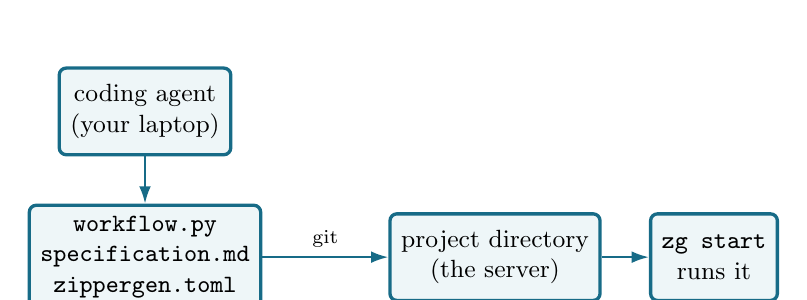
\begin{tikzpicture}[node distance=6mm]
  \node[zgstage] (agent) {coding agent\\(your laptop)};
  \node[zgstage, below=of agent] (files) {\texttt{workflow.py}\\\texttt{specification.md}\\\texttt{zippergen.toml}};
  \node[zgstage, right=16mm of files] (server) {project directory\\(the server)};
  \node[zgstage, right=of server] (run) {\texttt{zg start}\\runs it};
  \draw[zgflow] (agent) -- (files);
  \draw[zgflow] (files) -- node[above,font=\scriptsize]{git} (server);
  \draw[zgflow] (server) -- (run);
\end{tikzpicture}
\end{center}

Notice what does \emph{not} cross to the right. The coding agent stays on your
laptop. It wrote the workflow, but it is not part of the running application, and
the server never needs Claude, Codex, or an agent of any kind installed. The
server needs three things: ZipperGen, the project files, and its own
credentials.

On an ordinary Linux machine:

\begin{lstlisting}[style=shell]
git clone https://github.com/me/email-approval.git && cd email-approval
python3 -m venv .venv && source .venv/bin/activate
pip install zippergen

zg connector configure telegram approvals --chat-id 4242
zg connector assign User approvals

zg deploy --name production --no-start
zg start production
\end{lstlisting}

The credentials did not arrive with the clone, because they were never in it.
\texttt{configure} asks for the bot token, does not echo it, and stores it
outside the project. That is why cloning gives the server the routing without
giving it the secret.

The last two lines are the pair from the previous section, unchanged. Starting
probes the model and the connector first, so a token typed wrongly here fails
now rather than in the middle of an approval. On Linux \texttt{zg start}
installs a small \texttt{systemd} user service that restarts the workflow if it
fails. You never write that file, and \texttt{zg status}, \texttt{zg logs} and
\texttt{zg stop} manage it from here.

This is the point of the loop. The workflow you built does not finish, so
leaving it on a server is not a contrivance to show off a \texttt{deploy}
command. It is the only sensible place for it. Your laptop can close.

The mailbox here is a directory, which is enough to see the shape. Point
\texttt{next\_unread\_message} at a real inbox and nothing above changes.
\texttt{examples/call\_intake.py} is that workflow, reading Gmail and writing
to a spreadsheet.

\section{What you have}

\begin{center}
\begin{tabularx}{0.94\linewidth}{@{}lX@{}}
\toprule
\texttt{specification.md} & what it should do, in prose, maintained by you and your agent \\
\texttt{workflow.py} & the coordination, as visible Python \\
\texttt{zippergen.toml} & which model, which chat, committed, no secrets \\
\texttt{mailbox/} & where messages arrive, a real inbox on a real server \\
\bottomrule
\end{tabularx}
\end{center}

Three files and a directory, plus whatever your machine supplies: a model key
in the environment, a bot token typed once.

The thing worth remembering is the \texttt{Writer}. It learned about the loop,
because it has work to do inside it. It never learned about the approval,
because it has none. You wrote one protocol, and ZipperGen worked out what each
participant runs, and worked it out in a way that cannot deadlock. As the
workflow grows, with more participants, more loops and parallel regions, that is
what stops the coordination becoming the hard part.

\section{Where to go next}

\begin{itemize}
  \item \texttt{examples/diagnosis.py} has two reviewers who argue until they agree.
        A loop, and a decision inside it.
  \item \texttt{examples/call\_intake.py} reads a real mailbox and records to a
        real spreadsheet, runs as a service.
  \item \emph{Development and deployment guide} is the longer reference.
  \item \texttt{zippergen skill} prints what your coding agent is following. Worth
        reading once yourself.
\end{itemize}

\end{document}
